\documentclass[12pt,twoside,singlespace]{article}
\pagestyle{plain}

\usepackage{array, paralist, enumerate, amsmath, amsthm, amsfonts, amssymb, color, mathrsfs,comment}
%\usepackage{times}
\usepackage{geometry}
\usepackage{framed}
\usepackage{hyperref}
\usepackage{graphicx}
\usepackage{epstopdf}

\usepackage{tikz}
\usepackage{tkz-graph}
\usetikzlibrary{arrows,%
                shapes,positioning}

\definecolor{DarkBlue}{rgb}{0,0,0.8} 
\definecolor{DarkGreen}{rgb}{0,0.5,0.0} 
\definecolor{DarkRed}{rgb}{0.9,0.0,0.0} 

\usepackage[T1]{fontenc}
\usepackage[latin1]{inputenc}
%\usepackage[inline]{showlabels}

\numberwithin{equation}{section}
\newtheorem{thm}[equation]{Theorem}
\newtheorem{lem}[equation]{Lemma}
\newtheorem{cor}[equation]{Corollary}
\newtheorem{prop}[equation]{Proposition}
\newtheorem{construction}[equation]{Construction}

\theoremstyle{definition}
\newtheorem{definition}[equation]{Definition}
\newtheorem{ex}[equation]{Example}	
\newtheorem{remark}[equation]{Remark}
\newtheorem{prob}{Problem}

\newcommand{\BB}{\mathbf{B}}
\newcommand{\ZZ}{\mathbf{Z}}
\newcommand{\NN}{\mathbf{N}}
\newcommand{\RR}{\mathbf{R}}
\newcommand{\QQ}{\mathbf{Q}}
\newcommand{\CC}{\mathbf{C}}
\newcommand{\FF}{\mathbf{F}}
\newcommand{\N}{N}
\newcommand{\po}[2]{\mathfrak{po}^{#1|#2}}
\newcommand{\on}{\operatorname}
\newcommand{\ra}{\rightarrow}
\newcommand{\ul}{\underline}
\newcommand{\ol}{\overline}
\newcommand{\nin}{\noindent}

\newcommand{\simple}{\text{simple}}
\newcommand{\Img}{\on{Im}}
\newcommand{\con}{\on{Con}}
\newcommand{\dash}{\on{Dash}}

\geometry{verbose,letterpaper,tmargin=1in}

\newcommand{\Q}{\overline{q}}
\newcommand{\w}{\on{weight}}

\newcommand{\val}{\on{Val}}
\newcommand{\smon}{\mathbf{SMon}}
\newcommand{\clif}{\on{clif}}
\newcommand{\cl}{\mathbf{Cl}}
%\newcommand{\mov}[2]{\on{mov}_{#2}(#1)}
\newcommand{\inc}{\on{inc}}
\newcommand{\cut}[4]{#1 = #2 \amalg_{#4} #3}
\newcommand{\cutr}[3]{#1 \amalg_{#3} #2}
%\newcommand{\piece}[3]{#1(#2|#3)}
\newcommand{\piece}[3]{#1_{#3}}
\newcommand{\wt}{\on{wt}}

\newcommand{\com}[1]{\textcolor{red}{$[\star \star \star$ #1 $\star \star \star]$}}

%%%%%%%%%%%%%%%%%%%%%%%%%%%%%% LyX specific LaTeX commands.
%% Bold symbol macro for standard LaTeX users
\providecommand{\boldsymbol}[1]{\mbox{\boldmath $#1$}}

%%%%%%%%%%%%%%%%%%%%%%%%%%%%%% User specified LaTeX commands.
\renewcommand{\vec}[1]{\mathbf{#1}}

%\renewcommand{\labelenumi}{(\alph{enumi})}
%\renewcommand{\labelenumii}{(\roman{enumii})}

%\usepackage{babel}

\title{A proof of the H\"ubsch conjecture on constructing 2D Adinkras from 1D Adinkras}
\author{Kevin Iga and Yan X Zhang}

\begin{document}

\pagestyle{plain}

\maketitle

\section{Preliminaries}

\subsection{$1$-d Adinkras}
Adinkras in [references] will be referred to as $1$-d Adinkras in this paper, since they relate to supersymmetry in $1$ dimension.  We will review a definition of $1$-d Adinkras now.

\begin{definition}
Let $n$ be a non-negative integer.  A $1$-d Adinkra with $n$ colors is $(V,E,c,\mu,h)$ where
\begin{itemize}
\item $(V,E)$ is a finite undirected graph (called the underlying graph of the Adinkra) with vertex set $V$ and edge set $E\subset V\times V$,
\item $c:E\to \{1,\ldots,n\}$ is a map called the coloring,
\item $\mu:E\to \ZZ_2=\{0,1\}$ is a map called the dashing,
\item $h:V\to\ZZ$ is a map called the grading.
\end{itemize}

These are required to satisfy the following:
\begin{enumerate}
\item If $(v,w)\in E$, then $(w,v)\in E$.  Furthermore, $c(v,w)=c(w,v)$ and $\mu(v,w)=\mu(w,v)$.  Intuitively, the edges are undirected.
\item For every $v\in V$ and $c\in \{1,\ldots,n\}$, there exist exactly one $w\in V$ so that $(v,w)\in E$ and $c(v,w)=c$.
\item If $c_1$, $c_2\in \{1,\ldots,n\}$ with $c_1\not=c_2$, and $v\in V$, then there exist $w$, $x$, and $y\in V$ so that $(v,w)$, $(w,x)$, $(x,y)$, and $(y,v)\in E$, and $c(v,w)=c(x,y)=c_1$ and $c(w,x)=c(y,v)=c_2$ and $\mu(v,w)+\mu(w,x)+\mu(x,y)+\mu(y,v)\equiv 1\pmod{2}$.  Note that $\mu$ is called admissible if this last condition holds for every $v$, $w$, $x$ and $y$ that satisfy the above.
\item If $(v,w)\in E$, then $|h(v)-h(w)|=1$.
\end{enumerate}
\end{definition}
Note that in [Reference], there is also a bipartition of the vertices, where some vertices are represented by open circles and called bosons, and other vertices are represented by filled circles and called fermions.  This is not necessary to include in our definition, because a vertex $v$ is a boson if and only if $h(v)$ is even.

\subsection{The action of $\ZZ_2^n$ and the code}
Let $A$ be a $1$-d Adinkra with $n$ colors, with vertex set $V$.  For all $1\le i\le n$, define
\[q_i:V\to V\]
so that for all $v\in V$, $q_i(v)$ is the unique vertex joined to $v$ by an edge of color $i$.

\begin{definition}
\label{defn:homomorphism}
A graph homomorphism from a graph $(V_1,E_1)$ to a graph $(V_2,E_2)$ is a map $\phi:V_1\to V_2$ so that if $(v,w)\in E_1$ is an edge, then $(\phi(v),\phi(w))\in E_2$ is an edge.  If there is a coloring $c_1:E_1\to\{1,\ldots,n\}$ and a coloring $c_2:E_2\to\{1,\ldots,n\}$, we say that $\phi$ preserves colors if $c_1(v,w)=c_2(\phi(v),\phi(w))$.  If $\phi$ is bijective, we say that it is a graph isomorphism.
\end{definition}

\begin{prop}
\label{prop:qmap}
The map $q_i$ is a graph isomorphism from the underlying graph of $A$ to itself which preserves colors.  It is an involution and for all $i$, $j$, we have
\begin{equation}
q_i\circ q_j=q_j\circ q_i.\label{eq:commute}
\end{equation}
\end{prop}
\begin{proof}
The statement that $q_i$ is a graph homomorphism means that if $(v,w)$ is an edge in $A$, then so is $(q_i(v),q_i(w))$.  This follows from items 2 and 3 in the definition of an Adinkra above, using $j=c(v,w)$.

The fact that $q_i(q_i(v))=v$ for all $v\in V$ follows from item 2 in the definition.  This means that $q_i$ is an involution and in particular is an isomorphism.

The equation (\ref{eq:commute}) follows from item 3 of the definition when $i\not=j$ and is trivial when $i=j$.
\end{proof}

By combining the $q_1,\ldots, q_n$ maps, we can define an action of $\ZZ_2^n$ on the graph $(V,E)$ underlying the Adinkra in the following way:
\begin{definition}
The action of $\ZZ_2^n$ on the graph $(V,E)$ underlying the Adinkra is given on vertices by
\[(x_1,\ldots,x_n)v=q_1^{x_1}\circ\cdots\circ q_n^{x_n}(v).\]
\end{definition}

\begin{prop}
\label{prop:actioniso}
The above defines an action by graph isomorphisms that preserve colors.
\end{prop}
\begin{proof}
Acting on $v$ by $\vec{y}$ and then $\vec{x}$ gives
\begin{eqnarray*}
\vec{x}\vec{y}(v)
&=&q_1^{x_1}\circ\cdots\circ q_n^{x_n}\circ
q_1^{y_1}\circ\cdots\circ q_n^{y_n}(v)\\
&=&q_1^{x_1+y_1}\circ\cdots\circ q_n^{x_n+y_n}(v)
\end{eqnarray*}
by the commutativity shown in (\ref{eq:commute}), and where the exponents are taken modulo $2$, because each $q_i$ is an involution.  Therefore this is equal to
\[(\vec{x}+\vec{y})(v).\]

Proposition~\ref{prop:qmap} says that each $q_i$ is an isomorphism which preserves colors, and this action is a composition of such maps.
\end{proof}

\begin{definition}
A path is a finite sequence of edges of the form $((v_1,v_2),(v_2,v_3),\ldots,(v_{k-1},v_k))$.  The {\em color sequence} of the path is the sequence $(c(v_1,v_2),c(v_2,v_3),\ldots,c(v_{k-1},v_k))$.
\end{definition}

So if there is a path from $v$ to $w$ with color sequence $(i_1, \ldots, i_k)$, we have $w=q_{i_k}\circ \cdots\circ q_{i_1}(v)$.

\begin{prop}
\label{prop:colorpath}
Let $A$ be an Adinkra and let $v$ be a vertex of $A$.  Let $\sigma$ be a color sequence.  There exists a unique path in $A$ that starts at $v$ and has color sequence $\sigma$.
\end{prop}
\begin{proof}
This can be proved by induction on the length of $\sigma$, and using the fact that given a vertex $v_i$ of $A$, and a color $c_i$, there exists a unique vertex $v_{i+1}$ so that $(v_i,v_{i+1})$ is an edge of $A$ with color $c_i$.
\end{proof}

Now, define a map $s$ that takes a color sequence and returns an element of $\ZZ_2^n=\{0,1\}^n$ where the $i$-th coordinate is the number of times (modulo $2$) that color $i$ appears in the sequence. For example, $s(3,1,2,1) = 0110$.  Note that $s(\sigma)$ does not depend on the ordering of the color sequence $\sigma$.  This relates to paths in Adinkras because of the following:

\begin{prop}
\label{prop:colorendpath}
Let $A$ be an Adinkra.  Let $v$ be a vertex of $A$ and let $p$ be a path that begins at $v$.  Let $\sigma$ be the color sequence obtained from $p$.  Then the path $p$ ends at the vertex $s(\sigma)v$.
\end{prop}
\begin{proof}
If the color sequence is $\sigma=(i_1,\ldots,i_k)$, then the path $p$ ends at
$q_{i_k}\circ \cdots \circ q_{i_1}(v)$.  By the commutativity of the $q_i$, we can order them in non-decreasing order of $i_j$.  If any of the $q_i$ appear more than once, we use the fact that $q_i^2$ is the identity to reduce the number of $q_i$ modulo $2$.  The result is $s(\sigma)v$.
\end{proof}


\begin{cor}
\label{prop:pathands}
Let $A$ be an Adinkra.  Let $v$ be a vertex of $A$ and let $p$ and $p'$ be paths that begin at $v$.  Let $\sigma$ and $\sigma'$ be the color sequences obtained from $p$ and $p'$, respectively.  If $s(\sigma)=s(\sigma')$, then $p$ and $p'$ both end at the same point.
\end{cor}



\begin{definition}
Pick a vertex $v\in A$.  Define $C(A,v)$ to be the stabilizer of $v$ under this action of $\ZZ_2^n$.  Since it is a subgroup of $\ZZ_2^n$, $C(A,v)$ is a binary block code of length $n$.
\end{definition}

\begin{prop}
\label{prop:transitive}
The Adinkra $A$ is connected if and only if the $\ZZ_2^n$ action is transitive on the vertex set of $A$.
\end{prop}
\begin{proof}
Let $v$, $w$ be vertices of $A$.  If $A$ is connected, then there is a path in $A$ connecting $v$ to $w$.  Let $\sigma$ be the color sequence obtained from this path.  Then by Proposition~\ref{prop:colorendpath}, $s(\sigma)v=w$.

Conversely, suppose the action is transitive.  Let $v$ and $w$ be vertices of $A$.  Then there exists a $\vec{x}\in\ZZ_2^n$ so that $w=\vec{x}v$.  Write $\vec{x}=(x_1,\ldots,x_n)$ and construct a color sequence $\sigma$ by taking the $i$ for which $x_i=1$.  By Proposition~\ref{prop:colorpath}, there is a path starting at $v$ that has $\sigma$ as its color sequence.  By Proposition~\ref{prop:colorendpath}, this path ends at $s(\sigma)v=\vec{x}v=w$.
\end{proof}

\begin{prop}
If $A$ is connected, then the code $C(A,v)$ does not depend on $v$.
\end{prop}
\begin{proof}
Let $w\in V$.  By Proposition~\ref{prop:transitive}, there exists a $\vec{y}\in \ZZ_2^n$ so that $\vec{y} v=w$.

Let $\vec{x}\in \ZZ_2^n$.  The result follows from the sequence of equivalences:
\[\vec{x} w=w\Leftrightarrow \vec{x}\vec{y} v=\vec{y} v \Leftrightarrow \vec{y} \vec{x} v=\vec{y} v \Leftrightarrow \vec{x} v=v\]
\end{proof}

\begin{definition}
Given a connected Adinkra $A$, the code for $A$, called $C(A)$, is defined to be $C(A,v)$, where $v$ is a vertex of $A$.
\end{definition}




\begin{prop}
\label{prop:paths}
Let $A$ be an Adinkra.  Let $v$ be a vertex of $A$ and let $p$ and $p'$ be paths that begin at $v$.  Let $\sigma$ and $\sigma'$ be the color sequences obtained from $p$ and $p'$, respectively.  The paths $p$ and $p'$ end at the same vertex if and only if 
\[s(\sigma)-s(\sigma')\in C(A).\]
\end{prop}

\begin{proof}
Suppose $p$ and $p'$ end at the same vertex.  Then by Proposition~\ref{prop:colorendpath},
\[s(\sigma)v=s(\sigma')v.\]
Then\footnote{Note that in this sequence of equations, $\ZZ_2^n$ is written additively but the group action is written multiplicatively.}
\[v=s(\sigma')^{-1}(s(\sigma)v)=(s(\sigma)-s(\sigma'))v.\]
Thus, $s(\sigma)-s(\sigma')\in C(A)$.

Conversely, suppose $s(\sigma)-s(\sigma')\in C(A)$.  Then by reversing the above argument,
\[s(\sigma)v=s(\sigma')v\]
and thus, by Proposition~\ref{prop:colorendpath}, $p$ and $p'$ end at the same vertex.
\end{proof}

\subsection{Quotients of graphs and Adinkras}
\label{sec:quotient}
As we have seen, $\ZZ_2^n$, and therefore subgroups of $\ZZ_2^n$, act on Adinkras (more precisely, the underlying graphs), and it will be important to understand quotients of Adinkras by codes.

\begin{prop}
Let $\Gamma=(V,E)$ be a graph, and suppose $C$ is a group that acts on $V$ via graph isomorphisms.  Then $C$ acts on the set of edges in the following manner: if $c\in C$ and $(v,w)\in E$, then $c(v,w)=(cv,cw)$.
\end{prop}
\begin{proof}
The fact that $(cv,cw)$ is an edge follows directly from the definition of graph isomorphism.

The fact that this is a group action follows from the fact that $c(c'(v,w))=(c(c'(v)),c(c'(w)))=((cc')v,(cc')w)=(cc')(v,w)$.
\end{proof}

\begin{definition}
Suppose $C$ is a group that acts on a graph $(V,E)$ via graph isomorphisms.  We say that this group action is distant if for every non-identity group element $c\in C$, and every vertex $v\in V$, every path from $v$ to $cv$ is of length greater than 2.
\end{definition}

\begin{construction}
If a group $C$ acts on a graph $\Gamma=(V,E)$ via graph isomorphisms, then we create a graph $\Gamma/C$ as follows: let the set of vertices be the orbit space $V/C$.  Edges in $\Gamma/C$ are pairs $(Cv,Cw)$ where there exist $c_1, c_2\in C$ so that $(c_1v,c_2h)$ is an edge in $E$.
\end{construction}

\begin{prop}
\label{prop:distiso}
If, in the previous construction, the group action is distant, then there is a bijection from $E/C$ to the set of edges in $\Gamma/C$.
\end{prop}
\begin{proof}
For every orbit $C(v,w)$ of $C$ on the set of edges of $\Gamma$, there is an edge $(Cv,Cw)$.  This is an edge in $\Gamma/C$ because $(v,w)$ is an edge in $\Gamma$.  This assignment is independent of the choice of representative $(v,w)$ from $C(v,w)$ above since if $(v',w')$ is another representative, then there is a group element $c\in C$ so that $v'=cv$ and $w'=cw$.  Then $v'\in Cv$ and $w'\in Cw$ so that $Cv'=Cv$ and $Cw'=Cw$.

To see that this assignment is surjective follows directly from the definition: for every edge in $\Gamma/C$, there is an edge $(v,w)$ in $\Gamma$ that gets sent to it.

Now to prove that this is injective, suppose $(v,w)$ and $(v',w')$ are edges in $\Gamma$ and suppose $(Cv,Cw)=(Cv',Cw')$.  Then there are group elements $c_1$ and $c_2\in C$ so that $c_1v=v'$ and $c_2w=w'$.  On the other hand, there is an edge $(c_1v,c_1w)=(v',c_1w)$.  So $(v',c_1w)$ and $(v',c_2w)=(v',w')$ are edges in the graph.  Then $c_2c_1^{-1}$ is a group element that sends $c_1w$ to $c_2w$ but we have just constructed a path of length 2 from $c_1w$ to $c_2w$.  Since the group action is distant, we know that $c_2c_1^{-1}=1$ so that $c_1=c_2$.  Therefore $(v',w')=c_1(v,w)$.
\end{proof}

\begin{prop}
\label{prop:quotient}
If a group $C$ acts on an Adinkra $A$ using graph isomorphisms that preserve colors, and if the action is distant, then the coloring descends to a coloring on $A/C$ that satisfies those properties of Adinkras that relate to colors and not to dashings or grading.  That is, let $E/C$ denote the set of edges of $A/C$ as defined in the construction.  Then
\begin{enumerate}
\item If $(Cv,Cw)$ is an edge in $A/C$, then $(Cw,Cv)$ is also an edge.  Furthermore, $c(Cv,Cw)=c(Cw,Cv)$.
\item For every $Cv\in V/C$ and $c\in \{1,\ldots,n\}$, there exist exactly one $Cw\in V/C$ so that $(Cv,Cw)\in E/C$ and $c(Cv,Cw)=c$.
\item If $c_1$, $c_2\in \{1,\ldots,n\}$ with $c_1\not=c_2$, and $Cv\in V/C$, then there exist $Cw$, $Cx$, and $Cy\in V/C$ so that $(Cv,Cw)$, $(Cw,Cx)$, $(Cx,Cy)$, and $(Cy,Cv)\in E/C$, and $c(Cv,Cw)=c(Cx,Cy)=c_1$ and $c(Cw,Cx)=c(Cy,Cv)=c_2$
\end{enumerate}
\end{prop}
\begin{proof}
Since Proposition~\ref{prop:distiso} says that the edges of $A/C$ can be identified with $E/C$, and since the action of $C$ preserves colors, we can define the coloring on $E/C$, and thus, on the edges of $A/C$.

Property 1 follows from the construction of the edges of $A/C$.

Now we prove Property 2.  Let $Cv\in V/C$ and $c\in\{1,\ldots,n\}$.  Since $A$ is an Adinkra, there is exactly one vertex $w\in V$ so that $(v,w)\in E$ and $c(v,w)=c$.  There is thus an edge $(Cv,Cw)$ in $A/C$ that has color $c$.  To show uniqueness, suppose there is an $x\in V$ so that $(Cv,Cx)$ is in $A/C$ with color $c$.  This means there are group elements $\alpha,\beta\in C$ so that $(\alpha v,\beta x)$ is an edge of $A$ of color $c$.  By acting by $\alpha^{-1}$, we see that without loss of generality, $\alpha=1$.  Because $A$ is an Adinkra, there is a unique edge from $v$ that has color $c$.  So $\beta x = w$.  Therefore $x\in Cw$.

Now we prove Property 3.  Let $c_1$ and $c_2$ be two different colors, and $Cv\in V/C$.  Since $A$ is an Adinkra, there are vertices $w$, $x$, and $y$ in $V$ so that $(v,w)$, $(w,x)$, $(x,y)$ and $(y,v)\in E$ and $c(v,w)=c(x,y)=c_1$ and $c(w,x)=c(y,v)=c_2$.  Then $Cw$, $Cx$, and $Cy$ are the requisite vertices in $V/C$ with the given property.
\end{proof}


[Change notation?  Colors and codes are both $C$ and $c$...  Graphs are often $G$ but here they are $\Gamma$ because groups are often $G$.]

\begin{prop}
If $A$ is an Adinkra and $C$ acts on $A$ via graph isomorphisms, then there is a map
\[\pi:A\to A/C\]
 that is a graph homomorphism.  If the action is distant and if $C$ acts preserving colors, then $\pi$ preserves colors.
\end{prop}
\begin{proof}
Let $\pi(v)=vC$.  If $(v,w)$ is an edge in $A$, then $\pi(v)=vC$ and $\pi(w)=wC$ are connected via an edge in $A/C$ because of the existence of the edges $(v,w)$.

If the action is distant and $C$ acts preserving colors, then by Proposition~\ref{prop:quotient}, $A/C$ has a well-defined coloring defined by the following: if $(v,w)$ is an edge, then the color of $(vC,wC)$ is the color of $(v,w)$.
\end{proof}

\subsection{Quotienting the cube by a code}



The following $1$-d Adinkra was defined in [reference].
\begin{construction}
For any non-negative integer $n$, we have an Adinkra $I^n=(V,E,c,\mu,h)$ with
\begin{itemize}
\item $V=\ZZ_2^n=\{0,1\}^n$,
\item $E=\{(v,w)\,|\,\mbox{$v$ and $w$ differ in precisely one coordinate}\}$,
\item $c(v,w)$ is the coordinate where $v$ and $w$ differ,
\item $\mu(v,w)$ is the number of $1$s in $v$ before the coordinate $c(v,w)$, modulo $2$,
\item $h(v)=\wt(v)$ is the number of $1$s in $v$.
\end{itemize}
\end{construction}


\begin{definition}
Given $C$ a linear block code of length $n$, with all non-zero code words having weight greater than $2$, we can define a graph with edge colors $I^n/C$ as the orbit space of the action of $C\subset \ZZ_2^n$ on $I^n$ as a graph.
\end{definition}

Recall that $C$ acts via graph homomorphisms that preserve colors.  By Proposition~\ref{prop:quotient}, since code words are length at least $2$, the quotient $I^n/C$ makes sense as a graph with coloring.

\begin{thm}
\label{thm:cubemodulocode}
If $A$ is a connected Adinkra, then there is a graph isomorphism from $I^n/C(A)$ to $A$ that preserves colors.
\end{thm}
\begin{proof}
Choose a vertex $\overline{0}$ in $A$.  Let
\[\phi:I^n\to A\]
\[\phi(x_1,\ldots,x_n)=(x_1,\ldots,x_n)\overline{0}\]
where we are using the action of $\ZZ_2^n$ on $A$ as described above.

To see that this is a graph homomorphism, let $(x_1,\ldots,x_n)\in\ZZ_2^n$ and let $(y_1,\ldots,y_n)$ be another vertex connected to $(x_1,\ldots,x_n)$ with an edge of color $i$.  Then $y_j=x_j$ for all $j\not=i$ and $y_i=1-x_i$.  Then $(y_1,\ldots,y_n)\overline{0}=q_1^{y_1}\cdots q_n^{y_n}(\overline{0}) =  q_1^{x_1}\cdots q_i^{1-x_i}\cdots q_n^{x_n}(\overline{0})=q_i(q_1^{x_1}\cdots q_n^{x_n}(\overline{0}))=q_i(x_1,\ldots,x_n)$.  So $\phi(x_1,\ldots,x_n)$ and $\phi(y_1,\ldots,y_n)$ are connected by an edge of color $i$.  Note that this also shows that the graph homomorphism preserves colors.

We now prove that $\phi$ is surjective.  Since $A$ is connected, $\ZZ_2^n$ acts transitively on the vertex set of $A$, and so for any vertex $v$ of $A$, there exists an element $\vec{x} \in\ZZ_2^n$ so that $\vec{x} \overline{0}=v$.  Then $v=\phi(\vec{x})$.

To prove the isomorphism from $I^n/C(A)$ to $A$, we consider the necessary and sufficient conditions for $\phi(\vec{x})=\phi(\vec{y})$ for $\vec{x}$, $\vec{y}\in \ZZ_2^n$.  The condition $\phi(\vec{x})=\phi(\vec{y})$ is equivalent to $\phi(\vec{x}-\vec{y})\overline{0}=\overline{0}$.  This is equivalent to saying $\vec{x}-\vec{y}\in C(A)$.  Thus, the map $\phi$ descends to $I^n/C(A)$ and gives an isomorphism.
\end{proof}

In Reference ..., it was proved that if $A$ is a connected Adinkra, then $C(A)$ is a doubly even code.  Furthermore, if $C$ is any doubly even binary block code of length $n$, then there is an Adinkra with $C(A)=C$.



\begin{lem}
\label{lem:uniqueiso}
Given connected $1$-d Adinkras $A$ and $B$ and vertices $a$ of $A$ and $b$ of $B$, there is at most one graph isomorphism from $A$ to $B$ that preserves colors and sends $a$ to $b$.
\end{lem}
\begin{proof}
Suppose $\phi:A\to B$ is a graph isomorphism that preserves colors and sends $a$ to $b$.

Let $v$ be a vertex of $A$. Since $A$ is connected, there is a path from $a$ to $v$.  This produces a color sequence $\sigma$.  Since $\phi$ is a graph isomorphism that preserves colors, $\phi$ sends this path to a path in $B$ starting from $b$ with the same color sequence.  By Proposition~\ref{prop:colorpath}, there is only one path in $B$ with this property.  The end of this path is $\phi(v)$.
\end{proof}


Maybe delete this:


\begin{definition}
Let 
$A_1=(V_1,E_1,c_1,\mu_1,h_{L1},h_{R1})$
and
$A_2=(V_2,E_2,c_2,\mu_2,h_{L2},h_{R2})$
be 2-Adinkras with $(p,q)$ colors.  A homomorphism from $A_1$ to $A_2$ is a graph homomorphism
\[\phi:(V_1,E_1)\to (V_2,E_2)\]
that preserves colors and so that:
\begin{itemize}
\item If $v\in V_1$ then $h_{1L}(v)=h_{2L}(\phi(v))$.
\item If $v\in V_1$ then $h_{1R}(v)=h_{2R}(\phi(v))$.
\end{itemize}
Note that there is no condition on the dashings $\mu_1$ and $\mu_2$.
\end{definition}




\subsection{$2$-d Adinkras}
The notion of $2$-d Adinkras is described in Ref...[fill in references to various things].  We use a definition here that is equivalent to the one found in [some reference]: the proof is found in Appendix...[maybe?]

A $2$-d Adinkra is similar to a $1$-d Adinkra except that some colors are called ``left-moving'' and the other colors called ``right-moving''.  Edges are called ``left-moving'' if they are colored by left-moving edges, and right-moving otherwise.  Furthermore, there are two gradings, one that is affected by the left-moving edges and the other for the right-moving edges.

More formally,
\begin{definition}
Let $p$ and $q$ be non-negative integers.   A 2-d Adinkra with $(p,q)$ colors is a 1-d Adinkra $(V,E,c,\mu,h)$ with $p+q$ colors, and two grading functions $h_L:V\to \ZZ$ and $h_R:V\to \ZZ$ so that
\begin{itemize}
\item $h(v)=h_L(v)+h_R(v)$
\item if $(v,w)$ is a left-moving edge, then $|h_L(v)-h_L(w)|=1$ and $h_R(v)=h_R(w)$.  If $(v,w)$ is a right-moving edge, then $|h_R(v)-h_R(w)|=1$ and $h_L(v)=h_R(w)$.
\end{itemize}
\end{definition}


\subsection{Product of Adinkras}
One way to get $2$-d Adinkras is to take a product of two $1$-d Adinkras, where the first Adinkra uses only left-moving colors and the second Adinkra uses only right-moving colors.

\begin{construction}
\label{const:product}
Let $p$ and $q$ be non-negative integers.  Let $A_1=(V_1, E_1, c_1, \mu_1,h_1)$ be a $1$-d Adinkra with $p$ colors and let $A_2=(V_2, E_2, c_2, \mu_2,h_2)$ be a $1$-d Adinkra $q$ colors.  We can define the product of these Adinkras $A_1\times A_2$ as the following 2-Adinkra with $(p,q)$ colors:
\[A_1\times A_2=(V,E,c,\mu,h_L,h_R)\]
where
\begin{eqnarray*}
V&=&V_1\times V_2\\
E&=&E_1\cup E_2\mbox{ where}\\
E_1&=&\{((v_1,w),(v_2,w))\,|\,(v_1, v_2)\in E_1,\mbox{ and } w\in V_2\}\\
E_2&=&\{((v,w_1),(v,w_2))\,|\,v\in V, \mbox{ and }(w_1,w_2)\in E_2\}\\
c((v_1,w),(v_2,w))&=&c_1(v_1,v_2)\mbox{ for all $((v_1,w),(v_2,w))\in E_1$}\\
c((v,w_1),(v,w_2))&=&p+c_2(w_1,w_2)\mbox{ for all $(v,w_1),(v,w_2)\in E_2$}\\
h_L(v,w)&=&h_1(v)\\
h_R(v,w)&=&h_2(w)\\
\mu((v_1,w),(v_2,w))&=&\mu_1(v_1,v_2)\\
\mu((v,w_1),(v,w_2))&=&\mu_2(w_1,w_2)+h_1(v)\pmod{2}
\end{eqnarray*}
\end{construction}

\begin{prop}
Given Adinkras $A_1$ and $A_2$, $\mu$ is an admissible dashing for $A_1\times A_2$.  That is, given colors $c_1$ and $c_2$, and vertices $v$, $w$, $x$, and $y$ in $A_1\times A_2$, with edges $(v,w)$, $(w,x)$, $(x,y)$, and $(y,v)$ and colors $c(v,w)=c(x,y)=c_1$ and $c(w,x)=c(y,v)=c_2$, we have $\mu(v,w)+\mu(w,x)+\mu(x,y)+\mu(y,v)\equiv 1 \pmod{2}$.
\end{prop}
\begin{proof}
If $c_1$ and $c_2$ are both left-moving colors, then write $v=(v_1,z)$.  Then $w=(w_1,z)$, $x=(x_1,z)$, and $y=(y_1,z)$.  Then we have
\[\mu(v,w)+\mu(w,x)+\mu(x,y)+\mu(y,v)
= \mu_1(v_1,w_1)+\mu_1(w_1,x_1)+\mu_1(x_1,y_1)+\mu_1(y_1,v_1)\]
and the result follows from the fact that $\mu_1$ was an admissible dashing on $A_1$.

If $c_1$ and $c_2$ are both right-moving colors, then write $v=(z,v_2)$.  Then $w=(z,w_2)$, $x=(z,x_2)$, and $y=(z,y_2)$.  Then
\begin{eqnarray*}
&&\mu(v,w)+\mu(w,x)+\mu(x,y)+\mu(y,v)\\
&=& \mu_2(v_1,w_1)+h_1(z)+\mu_2(w_1,x_1)+h_1(z)+\mu_2(x_1,y_1)+h_1(z)+\mu_2(y_1,v_1)+h_1(z)
\end{eqnarray*}
which modulo $2$ is the same as 
\[\mu_2(v_1,w_1)+\mu_2(w_1,x_1)+\mu_2(x_1,y_1)+\mu_2(y_1,v_1).\]
The result follows from the fact that $\mu_2$ was an admissible dashing on $A_2$.


Now if $c_1$ is left-moving and $c_2$ is right-moving, then write $v=(v_1,v_2)$.  Then $w=(w_1,v_2)$, $x=(w_1,x_2)$, and $y=(v_1,x_2)$.  Now note that $v_1$ and $w_1$ are connected by an edge in $A_1$, so $h_1(v_1)$ and $h_1(v_2)$ differ by 1.  In particular, one of these is even and the other is odd.  Without loss of generality, suppose $h_1(v_1)$ is even.  Then $\mu(v,w)=\mu_1(v_1,w_1)$, $\mu(w,x)=\mu_2(v_2,x_2)+1$, $\mu(x,y)=\mu_1(w_1,v_1)$, and $\mu(y,v)=\mu_2(x_2,v_2)$, and we have
\begin{eqnarray*}
&&\mu_(v,w)+\mu(w,x)+\mu(x,y)+\mu(y,v)\\
&=&\mu_1(v_1,w_1)+\mu_2(v_2,x_2)+1+\mu_1(w_1,v_1)+\mu_2(x_2,v_2)\equiv 1\pmod{2}.
\end{eqnarray*}
\end{proof}


\begin{definition}
Let $p$ and $q$ be non-negative integers and let $n=p+q$.

Given a binary block code $C$ of length $p$, we can define a binary block code $\hat{C}$ of length $n$ by appending to the end of every code word in $C$ a string of $0$s of length $q$.

Likewise, given a binary block code $C$ of length $q$, we can define a binary block code $\check{C}$ of length $n$ by prepending to the beginning of every code word in $C$ a string of $0$s of length $p$.
\end{definition}

\begin{prop}
Let $A_1$ and $A_2$ be as above.  Then
\[C(A_1\times A_2)=\hat{C}(A_1)\oplus \check{C}(A_2).\]
\end{prop}
\begin{proof}
Let $(v_1,v_2)\in A_1\times A_2$.  Let $\vec{x}\in \ZZ_2^N$.  We can write $\vec{x}=\vec{x}_1+\vec{x}_2$ where $\vec{x}_1$ is zero in the last $q$ bits and $\vec{x}_2$ is zero in the first $p$ bits.  Now
\[\vec{x}(v_1,v_2)=(\vec{x}_1+\vec{x}_2)(v_1,v_2)=(\vec{x}_1v_1,\vec{x}_2v_2).\]
This means that $\vec{x}(v_1,v_2)=(v_1,v_2)$ if and only if $\vec{x}_1v_1=v_1$ and $\vec{x}_2 v_2=v_2$.

So $\vec{x}\in C(A_1\times A_2)$ if and only if $\vec{x}_1\in \hat{C}(A_1)$ and $\vec{x}_2\in \check{C}(A_2)$.
\end{proof}



\section{Structural Theorems}

In this section, we show that the coherence conditions of $2$-d adinkras force a lot of structure onto them. In particular, we can think of the vertices of $2$-d adinkras as arranged in a rectangle, with the stucture of the entire adinkra basically determined by a horizontal and a vertical ``slice'' of the picture.

\subsection{A $2$-d Adinkra Fits in a Rectangle}

Let the \emph{support} of a $2$-d adinkra (and/or its bigrading function $(h_L,h_R)$) be defined as the range of $(h_L,h_R)$, its bigrading function. Now, we show that the support of a connected $2$-d adinkra must form a rectangle in $\ZZ^2$.

Let $\sigma$ be a color sequence.  Let $l(\sigma)$ be a rearrangement of $\sigma$ that moves all the left-moving colors to the beginning, and let $r(\sigma)$ be a rearrangement of $\sigma$ that moves all the right-moving colors to the beginning. Thus, suppose $p = q = 2$, we have $l((3,1,2,1)) = (2,1,1,3)$ and $r((3,1,2,1)) = (3,2,1,1)$. We always have $s(l(\sigma)) = s(r(\sigma))$ in general, since $l(\sigma)$ and $r(\sigma)$ are just permutations of each other.

\begin{prop}
\label{prop:rectangle-completion}
Let $A$ be a connected Adinkra.  Suppose $(x_1,y_1)$ and $(x_2,y_2)$ are in the support of $A$.  Then $(x_1,y_2)$ and $(x_2,y_1)$ are also in the support of $A$.
\end{prop}
\begin{proof}
The statement that $(x_1,y_1)$ and $(x_2,y_2)$ is in the support of $A$ means that there exist vertices $v_1$ and $v_2$ of $A$ with $(h_L(v_1),h_R(v_1))=(x_1,y_1)$ and $(h_L(v_2),h_R(v_2))=(x_2,y_2)$, respectively.  Since $A$ is connected, there exists a path from $v_1$ to $v_2$.

Let $\sigma$ be the color sequence of this path.  Now $l(\sigma)$ is a color sequence that can be written as a concatenation $\alpha\beta$ where $\alpha$ is a color sequence only involving left-moving colors, and $\beta$ is a color sequence only involving right-moving colors.  Consider the vertex $u=s(\alpha)v_1$.  The color sequence $\alpha$ describes a path from $v_1$ to $u$ involving only left-moving colors, and so $h_R(u)=h_R(v_1)=y_1$.  The color sequence $\beta$ describes a path from $u$ to $v_2$ involving only right-moving colors, and so $h_L(u)=h_L(v_2)=x_2$.  To summarize, $(h_L(u),h_R(u))=(x_2,y_1)$.

Repeating this procedure with $r(\sigma)$ likewise provides a vertex $w$ with $(h_L(w),h_R(w))=(x_1,y_2)$.
\end{proof}

\begin{cor}
\label{cor:rectangle}
The support of a connected $2$-d adinkra is a rectangle.  That is, there exist integers $x_0$, $x_1$, $y_0$, and $y_1$ so that the support is
\[\{(x,y)\in\ZZ^2\,|\,x_0\le x\le x_1\mbox{ and }y_0\le y\le y_1\}\]
\end{cor}
\begin{proof}
Let $x_0$ and $y_0$ be the minima of the $x$ and $y$ coordinates, respectively, of the support of the Adinkra.  By Proposition~\ref{prop:rectangle-completion}, $(x_0,y_0)$ is in the support as well.

Likewise, if $x_1$ and $y_1$ are the maxima of the $x$ and $y$ coordinates, respectively, of the support of the Adinkra, then $(x_1,y_1)$ is in the support.  By Proposition~\ref{prop:rectangle-completion}, $(x_1,y_0)$ and $(x_0,y_1)$ are also in the support.

Since the Adinkra is connected, there must be paths from vertices with bigrading $(x_0,y_0)$ to vertices with bigrading $(x_1,y_1)$.  Since $h_L$ and $h_R$ can change by at most 1 along these paths, we see that for all $x_0\le x\le x_1$, there must exist $y_x$ so that $(x,y_x)$ is in the support.  Likewise for all $y_0\le y\le y_1$, there must exist $x_y$ so that $(x_y,y)$ is in the support.  By application of Proposition~\ref{prop:rectangle-completion} again, we get that $(x,y)$ is in the support for all $x_0\le x\le x_1$ and $y_0\le y\le y_1$.
\end{proof}

While it is neat that the vertices of a $2$-d adinkra $A$ line up nicely in a rectangle, we now show that there is even more regularity in its structure. Let $A_L$ (resp. $A_R)$ be the subgraphs of $A$ induced by left-moving (resp. right-moving) edges of $A$. %

\begin{lem}
\label{lem:qiso}
Let $A$ be a $2$-d Adinkra.  If $X$ is a connected component of $A_L$ and $i$ is a right-moving color, then there is a graph isomorphism between $X$ and $q_i(X)$ that preserves colors and $h_L$.  The analogous statement for $A_R$ also holds.
\end{lem}
\begin{proof}
Propostion~\ref{prop:qmap} states that $q_i$ is a graph isomorphism from the underlying graph of $A$ to itself that preserves colors.  If we restrict  $q_i$ to a connected component $X$ of $A_L$, the restricted map is an isomorphism from $X$ to $q_i(X)$ that preserves colors.

Since $i$ is a right-moving color, then for all vertices $v\in X$, $h_L(v)=h_L(q_i(v))$.
\end{proof}

\begin{lem}
\label{lem:qiconnected}
Let $A$ be a $2$-d Adinkra.  If $X$ is a connected component of $A_L$ and $i$ is a right-moving color, then $q_i(X)$ is the vertex set of a connected component of $A_L$. The analogous statement for $A_R$ also holds.
\end{lem}
\begin{proof}
Because the property of connectedness is preserved under graph isomorphism, we know that $q_i(X)$ is connected.  If we let $X'$ be the connected component of $A_L$ that contains $q_i(X)$, then the same argument proves that $q_i(X')$ is connected as well.  Since $X$ was assumed to be a connected component of $A_L$, we have that $q_i(X')\subseteq X$.  But since $q_i^2$ is the identity, $X=q_i^2(X)\subseteq q_i(X')\subseteq X$.  This means $q_i(X')=X$.  By the fact that $q_i^2$ is the identity, we also have $q_i(X)=X'$.
\end{proof}

\begin{prop}
\label{prop:kevin}
Let $A$ be a connected $2$-d Adinkra.  All connected components of $A_L$ (and respectively $A_R$) are isomorphic as graded posets.
\end{prop}
\begin{proof}
Let $X$ and $Y$ be two connected components of $A_L$. Pick vertices $x \in X$ and $y \in Y$. Since $A$ is connected, there is a path from $x$ to $y$ in $A$. Reorder the path so that the right-moving edges occur before the left-moving edges. Since the left-moving edges stay in $Y$, the right-moving edges alone take $x$ to a vertex $y' \in Y$.  The sequence of right-moving edges provides a color sequence $i_1,\ldots,i_k$, and thus, a sequence of compositions $q_{i_k}\circ\cdots\circ q_{i_1}$.  Now $q_{i_k}\circ\cdots\circ q_{i_1}(x)=y'$.  By repeated application of Lemma~\ref{lem:qiconnected}, we have that $q_{i_k}\circ\cdots\circ q_{i_1}(X)$ is a connected component of $A_L$ that contains $y'$, which is $Y$.  By repeated application of Lemma~\ref{lem:qiso}, we have an isomorphism of graphs that preserves colors and the grading $h_L$.
\end{proof}

With all this redundancy, what is the minimal amount of information required for us to understand a $2$-d adinkra? Proposition~\ref{prop:kevin} suggests we just need a single connected component for each direction to give us all the data; this turns out to basically be true, as we see in the next section.




\section{Main Theorem}

The main result of this section is the following theorem:
\begin{thm}
\label{thm:quotient}
Let $A$ be a connected $2$-d Adinkra.  Fix a vertex $\overline{0}$ in $A$ and let $A_L^0$ (resp. $A_R^0$) be the connected component of $A_L$ (resp. $A_R$) containing $\overline{0}$.

There is a binary block code $K$ of length $n$ so that $K\cap \hat{C}(A_L^0)=0$ and $K\cap \check{C}(A_R^0)=0$, and
\[C(A)=\hat{C}(A_L^0)\oplus \check{C}(A_R^0)\oplus K,\]
and there is a graph isomorphism
\begin{equation}
\label{eqn:quotientiso}
A\cong (A_L^0\times A_R^0)/K
\end{equation}
of the underlying graphs that preserves colors and the bigrading.
\end{thm}

Before we begin it will help to understand the relationship of the codes.
\begin{lem}
\label{lem:cplus}
\[\hat{C}(A_L^0)\oplus \check{C}(A_R^0) \subseteq C(A).\]
\end{lem}
\begin{proof}
Let $g\in\hat{C}(A_L^0)$ and $h\in \check{C}(A_R^0)$.  Then $g\overline{0}=\overline{0}$ because applying $g$ to $\overline{0}$ results in a path that lies completely inside $A_L^0$, and so the fact that $g\overline{0}=\overline{0}$ in $A_L^0$ (since $g\in \hat{C}(A_L^0)$) results in $g\overline{0}=\overline{0}$ in $A$.  Likewise $h\overline{0}=\overline{0}$.  So $(g+h)\overline{0}=g(h(\overline{0}))=\overline{0}$ and $g+h\in C(A)$.
\end{proof}

\begin{proof}[Proof of Theorem~\ref{thm:quotient}]
From Lemma~\ref{lem:cplus} and basic linear algebra, there exists a vector subspace $K$ of $\ZZ_2^N$ that is a vector space complement of
$\hat{C}(A_L^0)\oplus \check{C}(A_R^0)$ in $C(A)$.  That is,
\[C(A)=\hat{C}(A_L^0)\oplus \check{C}(A_R^0)\oplus K.\]
Then by Theorem~\ref{thm:cubemodulocode}, there is an isomorphism
\[i_1:A\cong I^n/C(A)\]
that preserves colors.  The proof of this began with choosing a special vertex in $A$, and we specify here that we should use our chosen vertex $\overline{0}$ of $A$.  This isomorphism then sends $\overline{0}$ to the coset containing $(0,\ldots,0)$ in $I^n/C(A)$.

We now note that
\begin{eqnarray*}
I^n/C(A)
&=&I^n/(\hat{C}(A_L^0)\oplus \check{C}(A_R^0)\oplus K)\\
&=&(I^n/(\hat{C}(A_L^0)\oplus \check{C}(A_R^0)))/ K\\
&=&(I^n/C(A_L^0 \times A_R^0))/ K
\end{eqnarray*}
and again apply Theorem~\ref{thm:cubemodulocode} to establish an isomorphism
\[i_2:(I^n/C(A_L^0 \times A_R^0))/ K\cong (A_L^0\times A_R^0)/K\]
that preserves colors and sends the coset of $(0,\ldots,0)$ to $(\overline{0},\overline{0})$.

We compose these isomorphisms to define
\[i_3:A\to (A_L^0\times A_R^0)/K\]
an isomorphism of graphs that preserves colors.

We now restrict $i_3$ to $A_L^0$.  It turns out that this sends every vertex $v$ of $A_L^0$ to $(v,\overline{0})$ in $(A_L^0\times A_R^0)/K$.  This can be seen by noting that both the restriction of $i_3$ to $A_L^0$ and the map sending $v$ to $(v,\overline{0})$ are graph isomorphisms that preserve colors and send $\overline{0}$ to $(\overline{0},\overline{0})$.  By Lemma~\ref{lem:uniqueiso}, such a map is unique.  Therefore, $i_3(v)=(v,\overline{0})$ for all vertices $v$ in $A_L^0$.  Likewise, a similar proof shows that if $v\in A_R^0$, then $i_3(v)=(\overline{0},v)$.

Now let $v$ be any vertex of $A$.  There is a path from $\overline{0}$ to $v$.  This gives a color sequence $\sigma$.  Consider the reordered color sequence $l(\sigma)$.  Write this as $\alpha\beta$ where $\alpha$ only involves left-moving colors and $\beta$ only uses right-moving colors.  Then define $x=s(\alpha)\overline{0}$.  Because $\alpha$ only involves left-moving colors, $x$ is in $A_L^0$.

Now since $\beta$ consists of right-moving colors, and connects $i_3(x)$ with $i_3(v)$, we have $h_L(i_3(v))=h_L(i_3(x))=h_L(x,\overline{0})=h_L(x)$.  This is $h_L(v)$ because $\beta$ only involves right-moving colors and connects $x$ with $v$.  Thus, $h_L(i_3(v))=h_L(v)$.

A similar proof shows that $h_R(i_3(v))=h_R(v)$.
\end{proof}






\begin{figure}[htb]
\begin{center}

\begin{tabular}{c|c}
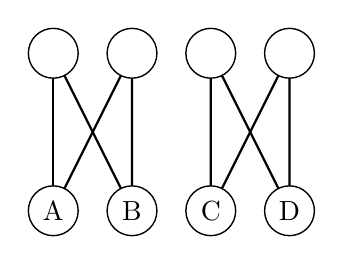
\begin{tikzpicture}[scale=0.10]
%\SetVertexNormal
\SetUpEdge[labelstyle={draw}]
\Vertex[x=0,y=0]{A}
\Vertex[x=10,y=0]{B}
\Vertex[x=20,y=0]{C}
\Vertex[x=30,y=0]{D}
\SetVertexNoLabel
\Vertex[x=0,y=20]{E}
\Vertex[x=10,y=20]{F}
\Vertex[x=20,y=20]{G}
\Vertex[x=30,y=20]{H}
\Edges(A, F, B, E, A)
\Edges(C, H, D, G, C)
\end{tikzpicture}
&
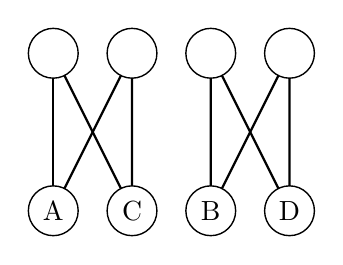
\begin{tikzpicture}[scale=0.10]
%\SetVertexNormal
\SetUpEdge[labelstyle={draw}]
\Vertex[x=0,y=0]{A}
\Vertex[x=10,y=0]{C}
\Vertex[x=20,y=0]{B}
\Vertex[x=30,y=0]{D}
\SetVertexNoLabel
\Vertex[x=0,y=20]{E}
\Vertex[x=10,y=20]{G}
\Vertex[x=20,y=20]{F}
\Vertex[x=30,y=20]{H}
\Edges(A, G, C, E, A)
\Edges(B, H, D, F, B)
\end{tikzpicture}
\end{tabular}
%\includegraphics[scale=0.5]{4cubefold}
\caption{Taking the product of the two adinkras here with the following identification gives a non-disconnected adinkra with 16 vertices. \label{fig:disconnected}}
\end{center}
\end{figure}

\subsection{Dashing}
We now consider the dashing.  It is too much to expect the dashing on $A_L^0\times A_R^0$ to agree with the dashing on $A$.  It is even generally untrue that the dashing on $A_L^0\times A_R^0$ is invariant under the quotienting action of $K$.  But if we allow vertex flips, then we can accomplish this.

\begin{definition}
Given an Adinkra $A$ (either $1$-d or $2$-d), and a vertex $v$ of $A$, the vertex flip is a new Adinkra $A'$ with the same vertices, edges, coloring, and grading(s) but a new dashing $\mu'$ so that
\begin{equation}
\mu'(e)=\begin{cases}
1-\mu(e),&\mbox{if $e$ is incident to $v$}\\
\mu(e),&\mbox{otherwise.}
\end{cases}
\end{equation}
\end{definition}

\begin{prop}
If $A$ is an Adinkra, then so is $A'$.
\end{prop}
\begin{proof}
Since the vertices, edges, coloring, and grading(s) are the same, the only thing to check is the admissibility of $\mu'$.  That is, given colors $c_1$ and $c_2$, and vertices $v$, $w$, $x$, and $y$, such that $(v,w)$ and $(x,y)$ are edges with color $c_1$ and $(w,x)$ and $(y,v)$ are edges with color $c_2$, that $\mu'(v,w)+\mu'(w,x)+\mu'(x,y)+\mu'(y,v)$ is odd.  If $v'$ is none of these vertices, then this sum is unchanged.  If $v'$ is any of these vertices, for instance, $v$, then $\mu'(v,w)$ and $\mu'(y,v)$ are both changed modulo $2$, so that the sum modulo $2$ is still unchanged.
\end{proof}

\begin{thm}
Let $A$ be a connected $2$-d Adinkra.  Let $\overline{0}$, $A_L^0$, $A_R^0$, and $K$ be as in Theorem~\ref{thm:quotient}.

Then there is a sequence of vertex flips on $A_L^0\times A_R^0$ so that the action of $K$ preserves the dashing, and the quotient by $K$ gives a dashing that agrees with the dashing on $A$ when compared via the isomorphism given in Theorem~\ref{thm:quotient}.
\end{thm}

Before proving this theorem, it is helpful to recognize that this theorem can be viewed as comparing two different dashings on $A_L^0\times A_R^0$.

Consider the dashing $\mu$ on $A$.  This restricts to $A_L^0$ and $A_R^0$, and via Construction~\ref{const:product}, this gives a dashing $\mu_1$ on $A_L^0\times A_R^0$.




At the same time, under the isomorphism (\ref{eqn:quotientiso}), the dashing $\mu$ on $A$ gets carried to $(A_L^0\times A_R^0)/K$.  The graph homomorphism
\[\pi:A_L^0\times A_R^0\to (A_L^0\times A_R^0)/K\]
pulls back the dashing to $\mu_2$ on $A_L^0\times A_R^0$.

\begin{prop}
The map $\pi$ above is a graph homomorphism.
\end{prop}
\begin{proof}

\end{proof}

\begin{prop}
$\mu_2$ is an admissible dashing.  That is, given colors $c_1$ and $c_2$, and vertices $v$, $w$, $x$, and $y$, with edges $(v,w)$, $(w,x)$, $(x,y)$, and $(y,v)$ and colors $c(v,w)=c(x,y)=c_1$ and $c(w,x)=c(y,v)=c_2$, we have $\mu_2(v,w)+\mu_2(w,x)+\mu_2(x,y)+\mu_2(y,v)\equiv 1 \pmod{2}$.
\end{prop}
\begin{proof}
Since $\pi$ is a graph homomorphism, and $c_1$, $c_2$, $v$, $w$, $x$, and $y$ are as above, then $\pi(v)$, $\pi(w)$, $\pi(x)$, and $\pi(y)$ satisfy the same condition.  If $\mu_2=\pi^*(\mu)$, then $\mu_2(v,w)+\mu_2(w,x)+\mu_2(x,y)+\mu_2(y,v)=\mu(\pi(v,w))+\mu(\pi(w,x))+\mu(\pi(x,y))+\mu(\pi(y,v))$ and the result follows from the fact that $\mu$ is an admissible dashing.
\end{proof}

In the language of cubical cohomology in [reference], what this theorem says is that $\mu_1-\mu_2$ is 0 in cohomology.

\begin{definition}
Given a path given by vertices $(v_0,\ldots,v_k)$, the parity of a dashing $\mu$ on the path is the following sum modulo 2:
\[\sum_{i=0}^{k-1} \mu(v_i,v_{i+1})\pmod{2}.\]
\end{definition}

\begin{lem}
The dashings $\mu_1$ and $\mu_2$ agree on $A_L^0\times \{\overline{0}\}$ and on $\{\overline{0}\}\times A_R^0$.
\end{lem}
\begin{proof}
The construction of $\mu_1$ gives all edges in $A_L^0\times\{\overline{0}\}$ as the same as in $A_L^0$ under the association of every edge $(v,w)$ with $((v,\overline{0}),(w,\overline{0}))$.  For $\mu_2$, consider that $i_3$ sends every vector $v\in A_L^0$ to $(v,\overline{0})$, and likewise any edges in $A_L^0$ will be sent to the corresponding edge in $A_L^0\times\{\overline{0}\}$.  Therefore $\mu_1$ and $\mu_2$ agree on $A_L^0\times\{\overline{0}\}$.  Likewise for $\{0\}\times A_R^0$.
\end{proof}

\begin{lem}
Given any cycle $(v_0,v_1,\ldots,v_k)$ with $v_0=v_k$, the parities of $\mu_1$ and $\mu_2$ on the cycle are equal.
\end{lem}
\begin{proof}
We first consider the case where $v_0=\overline{0}$.  Then there is a color sequence $\sigma$ from this.  We modify the path (and thereby modify the color sequence) by ``bubble sorting'' the colors.  Earlier, we noted that we could rearrange $\sigma$ to $l(\sigma)$ so that the left-moving colors were before the right-moving colors.  This can be more specifically done by a series of adjacent swaps of the type that sends the color sequence
\[(i_1,\ldots,i_{j-1},i_j,i_{j+1},i_{j+2},\ldots,i_k)\]
to
\[(i_1,\ldots,i_{j-1},i_{j+1},i_j,i_{j+2},\ldots,i_k).\]
A color swap of this type leads to a new path from $\overline{0}$, via Proposition~\ref{prop:colorpath}.  The path is unchanged up to $v_{j-1}$, but by the definition of Adinkras, property 3, the path returns to $v_{j+1}$ so it is only $v_j$ that has changed.  The effect on the parity of any dashing is, by property 3, to add $1$ modulo $2$.  In particular, $\mu_1$ and $\mu_2$ are both affected in the same way.

After a series of such color swaps, we rearrange $\sigma$ to $l(\sigma)$, and the path in question consists of left-moving edges, which remain in $A_L^0\times \{\overline{0}\}$, and then right-moving edges, which ends in $\overline{0}$, and so must be in $\{\overline{0}\}\times A_R^0$.  By the previous lemma, $\mu_1$ and $\mu_2$ are equal here, and so their parity on this modified path is the same.  Therefore, their parity on the original loop was the same.

Now we consider loops $p$ where $v_0\not=\overline{0}$.  Since $A_L^0\times A_R^0$ is connected, there is a path $p_0$ from $\overline{0}$ to $v_0$.  Take the path $p_0$, followed by $p$, then followed by $p_0^{-1}$ (meaning $p_0$ traversed in the opposite sense).  This is a loop starting and ending in $\overline{0}$, but the parity of a dashing is the same as that of $p$, since every new edge in $p_0$ is counterbalanced by a new edge in $p_0^{-1}$.  Therefore the parity of $\mu_1$ and $\mu_2$ agree on all loops.
\end{proof}

\begin{definition}
Let $V'\subset V$ and let $\mu$ be a dashing.  Then we can define a vertex flip of $\mu$ by $V'$ to be a dashing $\psi_{V'}(\mu)$ so that
\[\psi_{V'}(\mu)(e)=\mu(e)+i(e,V')\pmod{2},\]
where $i(e,V')$ is the number of elements of $V'$ that are incident with the edge $e$.
\end{definition}

Note that the property 3 of Adinkras is unchanged if we use $\psi_{V'}(\mu)$ instead of $\mu$, so the result of replacing $\mu$ with $\psi_{V'}(\mu)$ is still an Adinkra.

\begin{lem}
If $\mu_1$ and $\mu_2$ have the same parity on all cycles, then there is a set of vertices $V'\subset V$ so that $\mu_2=\psi_{V'}(\mu_1)$.
\end{lem}

Two proofs: one using cohomology, one using spanning trees.




% To prove: \mu_1 is Adinkraic dashing
% \mu_2 is an Adinkraic dashing




\section{ESDE Codes}
Let $p$ and $q$ be non-negative integers so that $p+q=n$, and let $C$ be a linear block code of length $n$.  For every element $\vec{x}=(x_1,\ldots,x_n)\in\ZZ_2^n$, we define $\wt_L(\vec{x})$ to be the number of $1$s of $(x_1,\ldots,x_p)$ in the first $p$ components, and $\wt_R(\vec{x})$ to be the number of $1$s of $(x_{p+1},\ldots,x_n)$ in the last $q$ components.  Then $\wt(\vec{x})=\wt_L(\vec{x})+\wt_R(\vec{x})$.


Define a \emph{even-split doubly-even (ESDE) code} of length $(p,q)$ to be a doubly-even code of length $n$ so that every word $\vec{x}$ in the code has $\wt_L(\vec{x})$ and $\wt_R(\vec{x})$ even.

Recall that $1$-d chromotopologies are in bijection with quotients of the hamming cube $I^n$ by a doubly-even code $C$, so any adinkra $A$ has a well-defined associated code $C(A)$ that is uniquely determined by just the graph structure of the adinkra. Our goal is to show that ESDE codes are exactly the codes that appear for $2$-d adinkras. To do this, we introduce a special family of $2$-d adinkras.

In [references], there was a class of $1$-d Adinkras that were particularly easy to construct and study, called {\em Valise} Adinkras, whose height function had values in two adjacent integers (usually $0$ and $1$).  By analogy, given a ESDE code, we construct a $2$-d Adinkra called the {\em Valise 2-d Adinkra} that has support in a $2\times 2$ square.


\begin{construction}
\label{cons:valise}
Let $C$ be an ESDE code.  We will describe a construction that provides a $2$-d Adinkra with code $C$, called the {\em Valise 2-d Adinkra}.

$C$ is doubly-even, so there exists a connected $1$-d Adinkra $A$ with code $C(A) = C$.  [reference: this was a construction somewhere else]

We now wish to define a bigrading $(h_L,h_R)$.  To do this we do not use the grading $h$ that comes from the $1$-d Adinkra $A$.  Instead, fix a vertex $\overline{0}$ of $A$.  For every vertex $v$ of $A$, pick a path from $\overline{0}$ to $v$.  This produces a color sequence $d$.  Define $h_L(v)$ to be the number modulo 2 of left-moving colors in $d$ and likewise $h_R(v)$ is the number modulo 2 of right-moving colors in $d$.  These functions are well-defined if every path from $\overline{0}$ to $v$ has the same parity in number of left-moving colors and in number of right-moving colors.  This occurs if and only if every loop starting from $\overline{0}$ has an even number of left-moving colors and an odd number of right-moving colors.  If $C$ is ESDE, then this is the case.
\end{construction}

\begin{thm}
This construction gives a $2$-d Adinkra with code $C$.
\end{thm}
\begin{proof}
By construction, $A$ is a $1$-d Adinkra with code $C$.  The only thing left to check is whether the $h_L$ and $h_R$ that are defined satisfy the correct properties on edges.

Let $(v,w)$ be a left-moving edge in the Adinkra $A$.  Then the color of the edge is left-moving and so $h_L(v)\not=h_L(w)$ and $h_R(v)=h_R(w)$.  Since the possible values for $h_L$ and $h_R$ are $0$ and $1$, it follows that $|h_R(v)-h_R(w)|=1$.

The proof is similar for right-moving edges.
\end{proof}




\begin{figure}[htb]
\begin{center}

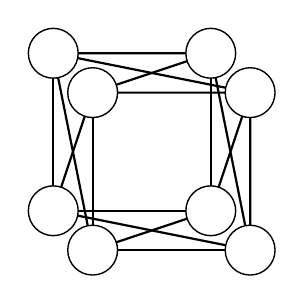
\begin{tikzpicture}[scale=0.10]
%\SetVertexNormal
\SetVertexNoLabel
\SetUpEdge[labelstyle={draw}]
\Vertex[x=0,y=0]{A}
\Vertex[x=-5,y=5]{H}
\Vertex[x=0,y=20]{C}
\Vertex[x=-5,y=25]{B}
\Vertex[x=15,y=5]{D}
\Vertex[x=20,y=0]{E}
\Vertex[x=20,y=20]{G}
\Vertex[x=15,y=25]{F}
\Edges(A,B,G)
\Edges(B,H,C)
\Edges(G,D)
\Edges(C,A,D,H,E,A)
\Edges(D,F,C,G,E,F,B)
\end{tikzpicture}
\caption{A valise $2$-d adinkra that cannot be put into non-valise form.\label{fig:tight valise}}
\end{center}
\end{figure}

\begin{thm}
\label{thm:esde}
For a code $C \subset \ZZ_2^n$, there exists a $2$-d adinkra $A$ with $C(A) = C$ if and only if $C$ is a ESDE code.
\end{thm}
\begin{proof}
Suppose $C(A) = C$ for some $2$-d Adinkra $A$. We know that $C$ is doubly-even. Consider any codeword $\alpha \in C$. Starting at $\overline{0} \in A$, moving by a path corresponding to $\alpha$ must end up back at $\overline{0}$. In particular, it must use an even number of left-moving (resp. right-moving) edges since each of such edge changes the $h_L$ (resp. $h_R$) by $1$ in absolute value. Thus, $C$ must be ESDE.

Conversely, given an ESDE code $C$, we can use Construction~\ref{cons:valise} to get a $2$-d Adinkra with code $C$.
\end{proof}


\subsection{Finding $K$}
Given a $2$-d Adinkra $A$, with special basepoint $\overline{0}$ and corresponding $A_L^0$ and $A_R^0$, there remains the question of finding the code $K$.  Recall that
\[C(A)=\hat{C}(A_L^0)\oplus\check{C}(A_R^0)\oplus K.\]
There is some choice involved in defining $K$; it merely has to be a vector space complement to
\[C'=\hat{C}(A_L^0)\oplus\check{C}(A_R^0).\]
$K$ will more naturally be defined as $C(A)/C'$, though computationally we can choose a representative to be $K$.


Let $V^0=A_L^0\cap A_R^0$.  Now for every $v\in V^0$, we have $h_L(v)=h_L(\overline{0})$ and $h_R(v)=h_R(\overline{0})$ so in particular, $V^0$ has no edges; only vertices.

We construct a bijection between $V^0$ and $C(A)/C'$.

\begin{construction}
\label{cons:findk}
For every $v\in V^0$, there is a path $p_L$ from $\overline{0}$ to $v$ in $A_L^0$ and a path $p_R$ from $v$ to $\overline{0}$ in $A_R^0$.  These paths give color sequences $\sigma_L$ and $\sigma_R$ with $\beta_L=s(\sigma_L)$ and $\vec{x}_R=s(\sigma_R)$ so that $\vec{x}_L$ is $0$ in the last $q$ coordinates and $\vec{x}_R$ is $0$ in the first $p$ coordinates.  Since the paths $p_L$ and $p_R$ form a loop in $A$, we know that $\vec{x}_L+\vec{x}_R\in C(A)$.

The paths $p_L$ and $p_R$ are not canonical, but if $p'_L$ and $p'_R$ are other paths with those properties, then $p_L(p'_L)^{-1}$ is a loop in $A_L^0$ from $\overline{0}$.  Let $\sigma'_L$ and $\sigma'_R$ be the corresponding color sequences, then $s(\sigma_L)+s(\sigma'_L)\in C(A_L^0)$.  Likewise, $s(\sigma_R)+s(\sigma'_R)\in C(A_R^0)$.

Thus, the choice of $\vec{x}_L+\vec{x}_R$ is well-defined modulo $C'=\hat{C}(A_L^0)\oplus \check{C}(A_R^0)$.  This provides a map from $V^0$ to $K=C(A)/C'$.
\end{construction}

\begin{thm}
\label{thm:findk}
The above construction provides a bijective map
\[\Phi:V^0\to C(A)/C'\]
\end{thm}
\begin{proof}

We now prove this map is bijective by providing its inverse.  Suppose $\vec{x}\in C(A)$.  Then by Proposition~\ref{prop:colorpath}, there is a loop in $A$ starting at $\overline{0}$ that follows the colors indicated by $\vec{x}$.  This gives a color sequence $\sigma$ so that $s(\sigma)=\vec{x}$.  Write $l(\sigma)=\alpha\beta$ where $\alpha$ only involves left-moving colors and $\beta$ only involves right-moving colors.  Let $v=s(\alpha)\overline{0}$.  Since $\alpha$ only involves left-moving colors, we have $v\in A_L^0$.  Since $s(\beta)v=\overline{0}$, and $\beta$ only involves right-moving colors, we have that $v\in A_R^0$.  Therefore $v\in V^0$.  Note that $v$ does not depend on the order of the left-moving colors in the color sequence, as long as they all come before the right-moving colors.  Thus we have a map
\[\Psi: C(A)  \to V^0.\]

Now suppose $\vec{y}\in \hat{C}(A_L^0)$ and $\vec{z}\in \check{C}(A_R^0)$.  We consider how the loop in the previous paragraph changes if we replace $\vec{x}$ with $\vec{x}+\vec{y}+\vec{z}$.  We use Proposition~\ref{prop:colorpath} to create a loop $p_1$ in $A_L^0$ that starts at $\overline{0}$ and follows the colors indicated by $\vec{y}$.  Then let $p_2$ be the path from $\overline{0}$ following the colors indicated by $s(\alpha)$ and $p_3$ the path that continues this using $s(\beta)$.  Finally, let $p_4$ be the path from there using the colors of $\vec{z}$.  By Proposition~\ref{prop:colorpath}, since $p_2$ starts from $\overline{0}$, it must still end at the same point $v$.  Therefore the map $\Psi$ descends to a map
\[\tilde{\Psi}:C(A)/C' \to V^0.\]

We now show that this function is the inverse of Construction~\ref{cons:findk}.  Let $v\in V^0$.  The construction gives a path $p_L$ of left-moving edges starting from $\overline{0}$ and ending in $v$ and a path $p_R$ of right-moving edges starting from $v$ to $\overline{0}$.  Composing these paths gives the result of the Construction.  Then we apply $\tilde{\Psi}$.  This takes the code word and finds the loop, which by Proposition~\ref{prop:colorpath} must be $p_Lp_R$.  Then $\Psi$ of the code word is the vertex at the end of $p_L$, which is $v$.


[show the other composition is the identity]

\end{proof}


To do:

See if there is a place for a Lemma that says you can reorder a path so left colors come first.


\appendix




\section{Representations of supersymmetry}
The $1$-d $n$-extended supersymmetry algebra is a superalgebra consisting of an even operator $H$ and $n$ odd operators $Q_1, \ldots, Q_n$ with the following relations:
\begin{eqnarray}
\label{eqn:susy1d1}
[H,Q_i]&=&0\\
\label{eqn:susy1d2}
\{Q_i,Q_j\}&=&2\delta_{ij}H
\end{eqnarray}

\begin{construction}
\label{cons:susy1d}
Given a $1$-d Adinkra $A=(V,E,c,\mu,h)$ with $n$ colors, we can find a representation $R(A)$ of the $1$-d $n$-extended supersymmetry algebra as follows:
\begin{itemize}
\item Let $R_0$ be the real vector space generated by $V$.  That is, $R_0$ is the set $\{f:V\to \RR\}$ viewed as a vector space with function addition and scalar multiplication.  There is a basis given by $\{b_v\,|\,v\in V\}$ with $b_v(v)=1$ and $b_v(w)=0$ if $v\not=w$.
\item Let $R(A)=R_0\otimes_\RR \RR[H]$.  This is a representation of $\RR[H]$ with $H(b\otimes H^k)=b\otimes H^{k+1}$, and $H$ extends to all of $R$ linearly.
\item If $v\in V$ and $w=q_i(v)$, then
\[Q_i(b_v\otimes H^k)=(-1)^{\mu(v,w)} b_w\otimes H^{k+\frac12(1-h(w)+h(v))}\]
Extend $Q_i$ to all of $R(A)$ linearly.
\item There is a $\ZZ_2$ grading of $R(A)$: let the $\ZZ_2$ grading of $b_v\otimes H^k$ be $h(v)\pmod{2}$.
\end{itemize}
\end{construction}
Note that the exponent of $H$, $i+\frac12(1-h(w)+h(v))$, is an integer because $|h(w)-h(v)|=1$.

\begin{prop}
\label{prop:rep1}
$R$ is a representation of the $1$-d supersymmetry algebra.
\end{prop}
\begin{proof}
First note that each $Q_i$ acts by changing the $\ZZ_2$ grading and $H$ does not.  Therefore the $Q_i$ are odd operators and $H$ is an even operator.

Since $b_v$ is a basis for $R_0$, $b_v\otimes 1$ is a generator of $R$ as an $\RR[H]$-module.  It suffices, then, to prove (\ref{eqn:susy1d1})--(\ref{eqn:susy1d2}) for $b_v\otimes 1$.

If $q_i(v)=w$, then
\begin{eqnarray*}
Q_i(H(b_v\otimes H^k))&=&Q_i(b_v\otimes H^{k+1})\\
&=&(-1)^{\mu(v,w)}b_w\otimes H^{k+1+\frac12(1-h(w)+h(v))}\\
&=&H((-1)^{\mu(v,w)}b_w\otimes H^{k+\frac12(1-h(w)+h(v))})\\
&=&H(Q_i(b_v\otimes H^k))
\end{eqnarray*}

We also have
\begin{eqnarray*}
Q_i(Q_i(b_v\otimes H^k))
&=&Q_i((-1)^{\mu(v,w)} b_w\otimes H^{k+\frac12(1-h(w)+h(v))})\\
&=&(-1)^{\mu(v,w)} (-1)^{\mu(w,v)} b_v\otimes H^{k+\frac12(1-h(w)+h(v))+\frac12(1-h(v)+h(w))}\\
&=&b_v\otimes H^{k+1}\\
&=&H(b_v\otimes H^{k})
\end{eqnarray*}

Now consider $\{Q_i,Q_j\}$ where $i\not=j$.  Let $w=q_i(v)$ and $x=q_j(w)$ and $y=q_i(x)$.  Then from Property 3 of Adinkras, $v=q_j(y)$.
\begin{eqnarray*}
Q_i(Q_j(b_v\otimes H^k))
&=&Q_i((-1)^{\mu(v,y)}b_y\otimes H^{k+\frac12(1-h(y)+h(v))})\\
&=&(-1)^{\mu(v,y)+\mu(y,x)}b_x\otimes H^{k+\frac12(1-h(y)+h(v))+\frac12(1-h(x)+h(y))})\\
&=&(-1)^{\mu(v,y)+\mu(y,x)}b_x\otimes H^{k+\frac12(2-h(x)+h(v))})
\end{eqnarray*}
while
\begin{eqnarray*}
Q_j(Q_i(b_v\otimes H^k))
&=&Q_j((-1)^{\mu(v,w)}b_w\otimes H^{k+\frac12(1-h(w)+h(v))})\\
&=&(-1)^{\mu(v,w)+\mu(w,x)}b_x\otimes H^{k+\frac12(1-h(w)+h(v))+\frac12(1-h(x)+h(w))})\\
&=&(-1)^{\mu(v,w)+\mu(w,x)}b_x\otimes H^{k+\frac12(2-h(x)+h(v))})
\end{eqnarray*}
Since
\[\mu(v,w)+\mu(w,x)+\mu(x,y)+\mu(y,v)\equiv 2\pmod{2},\]
we have
\[Q_jQ_i(b_v\otimes H^k)=-Q_iQ_j(b_v\otimes H^k).\]
\end{proof}

\begin{definition}
A representation $M$ of $1$-d $n$-extended supersymmetry algebra is called adinkraic if there exists a $1$-d Adinkra $A$ with $n$ colors so that $R(A)=M$ in Construction~\ref{cons:susy1d}.
\end{definition}

Though not relevant for our theorems, one can notice that the grading $h$ provides a grading to $R$ in the following way: the mass dimension of $b_v\otimes H^k$ is $k+\frac12 h(v)$.  Then $H$ has grading $1$ and each $Q_i$ has grading $\frac12$.

\subsection{Representations of $2$-d supersymmetry}
The $2$-d $(p,q)$-extended supersymmetry algebra has two even operators $H$ and $P$, and $n$ odd operators $Q_1,\ldots, Q_n$, with the first $p$ being viewed as ``left-moving'' and the remaining $q=n-p$ being viewed as ``right-moving''.  $H$ and $P$ commute with everything, while
\[
\{Q_i, Q_j\}=\begin{cases}
2\delta_{ij}(H+ P),&\mbox{ if $i\le p$}\\
2\delta_{ij}(H- P),&\mbox{ if $i> p$}\\
\end{cases}
\]
We define $P_- = H+ P$ and $P_+=H-P$.

\begin{construction}
Given a $2$-d Adinkra $A=(V,E,c,\mu,h_L,h_R)$ with $(p,q)$ colors, we get a representation of the $2$-d $(p,q)$-extended supersymmetry algebra as follows:
\begin{itemize}
\item Let $R_0=\{f:V\to\RR\}$ as a vector space.  Again, for every $v\in V$ define $b_v(v)=1$ and $b_v(w)=0$ if $v\not=w$.
\item Let $R(A)=R_0\otimes_\RR \RR[P_-,P_+]$ as a free $\RR[P_-,P_+]$-module.
\item If $i\le p$, and $w=q_i(v)$, then define
\[Q_i(b_v\otimes P_-^k P_+^l)=
(-1)^{\mu(v,w)}b_w\otimes P_-^{k+\frac12(1-h_L(w)+h_L(v))}P_+^l \]
\item If $i>p$ then
\[Q_i(b_v\otimes P_-^k P_+^l)=
(-1)^{\mu(v,w)}b_w\otimes P_-^k P_+^{l+\frac12(1-h_L(w)+h_L(v))} \]
\item There is a $\ZZ_2$ grading of $R(A)$: let the $\ZZ_2$ grading of $b_v\otimes H^k$ be $h_L(v)+h_R(v)\pmod{2}$.
\end{itemize}
\end{construction}

\begin{prop}
\label{prop:rep2}
$R(A)$ is a representation of the $2$-d $(p,q)$-extended supersymmetry algebra.
\end{prop}
\begin{proof}
The proof is largely the same as Proposition~\ref{prop:rep1}.
\end{proof}

\begin{construction}
Let $R_L$ be a representation of $1$-d $p$-extended supersymmetry and $R_R$ be a representation of $1$-d $q$-extended supersymmetry.  Then we define
\[R_L\otimes R_R\]
a representation of $2$-d $(p,q)$ supersymmetry as follows.
\begin{itemize}
\item For $i\le p$, $Q_i(a\otimes b)=Q_i(a)\otimes b$.
\item For $i>p$, $Q_i(a\otimes b)=(-1)^{|a|}a\otimes Q_{i-p} b$.
\item $H(a\otimes b)=H a\otimes b + a\otimes Hb$
\item $P(a\otimes b)=Pa \otimes b + a\otimes Pb$
\end{itemize}
Here $|a|$ means the $\ZZ_2$ grading of the element $a$ in $R_L$.
\end{construction}

\begin{prop}
$R_L\otimes R_R$ is a representation of $2$-d $(p,q)$-extended supersymmetry.
\end{prop}
\begin{proof}
This is standard in the SUSY literature.
\end{proof}

\begin{prop}
Let $A_L$ and $A_R$ be $1$-d Adinkras with $p$ and $q$ colors respectively.  Let $R(A_L)$ and $R(A_R)$ be the representations of $1$-d supersymmetry obtained from $A_L$ and $A_R$, respectively, by Construction~\ref{cons:susy1d}.  Then there is an isomorphism of representations of $2$-d $(p,q)$-extended supersymmetry
\[R(A_L)\otimes R(A_R) \cong R(A_L\times A_R)\]
\end{prop}
\begin{proof}
Let $v\in A_L$ and $w\in A_R$.  The isomorphism sends $(b_v\otimes H^k)\otimes (b_w\otimes H^l)$ to $b_{(v,w)}\otimes P_-^{k}P_+^l$.
\end{proof}

\begin{prop}
Let $A$ be an Adinkra and let $v$ be a vertex of $A$.  Let $A'$ be the Adinkra obtained by doing a vertex flip on $v$.  Then there is an isomorphism from $R(A)$ and $R(A')$.
\end{prop}
\begin{proof}
Let $\Phi$ be the linear map that sends $b_v\otimes H^k$ to $-b_v\otimes H^k$, and for every $w\not=v$, $b_w\otimes H^k$ to $b_w\otimes H^k$.

Let $w=q_i(v)$.  Now $Q_i(\Phi(b_v\otimes H^k))=Q_i(-b_v\otimes H^k)=-(-1)^{\mu(v,w)}b_w H^{k+\frac12(1-h(w)+h(v)}=(-1)^{\mu'(v,w)}b_w H^{k+\frac12(1-h(w)+h(v)}=\Phi(Q_i(b_v\otimes H^k))$.

etc. etc. [This is tedious.]
\end{proof}

\begin{prop}
Let $A=(V,E,c,\mu,h_L,h_R)$ and $A'=(V,E,c,\mu,h_L,h_R)$ be $2$-d Adinkras and let $f:V\to V'$ be a graph homomorphism that preserves coloring, dashing, and gradings.  Then the linear map
\[f_*:R(A)\to R(A')\]
\[f_*(b_v\otimes P_-^kP_+^l)=b_{f(v)}\otimes P_-^kP_+^l\]
is a homomorphism of representations.
\end{prop}
\begin{proof}
The map $f_*$ commutes with $P_+$ and $P_-$.  If $i$ is a left-moving color and $q_i(v)=w$, then $q_i(f(v))=f(w)$ and
\[f_*(Q_i(b_v\otimes P_-^kP_+^l))=f_*((-1)^{\mu(v,w)}b_w\otimes P_-^{k+\frac12(1-h_L(w)+h_L(v))}P_+^l\]
while
\[Q_i(f_*(b_v\otimes P_-^kP_+^l))=Q_i(b_{v'}\otimes P_-^kP_+^l)
=(-1)^{\mu'(f(v),f(w))}b_{f(w)}\otimes P_-^{1-h'_L(f(w))-h'_R(f(v))}P_+^l\]
which is the same thing if $f$ preserves dashing and gradings.

Likewise if $i$ is a right-moving color.
\end{proof}

\begin{thm}
If $A$ is a $2$-d Adinkra with $(p,q)$ colors, then 
\[R(A)=(R(A_L^0)\otimes R(A_R^0))/M\]
where $M$ is a submodule.
\end{thm}
\begin{proof}
From the main theorem Theorem~\ref{thm:quotient},
\[A=(A_L^0\times A_R^0)/K\]
and in particular there is a graph homomorphism
\[f:A_L^0\times A_R^0\to A\]
that is surjective and preserves coloring, dashing, and gradings.  Take the coresponding linear map
\[f_*:R(A_L^0\times A_R^0)\to R(A)\]
and let $M$ be the kernel of this map.  Composed with the isomorphism
\[R(A_L^0)\otimes R(A_R^0)\cong R(A_L^0\times A_R^0)\]
we have the isomorphism.
\end{proof}


\section{Equivalence with other notions of $2$-d Adinkras}


If I read Tristan's stuff right, we can completely translate the combinatorial rules to: a \emph{2-d adinkra} (of dimension $n$) is a finite simple connected graph $A$ such that:
\begin{itemize}
\item It is an $1$-d adinkra (with the associated ranking, dashing, etc.).
\item It has $p + q = n$ colors, where the first $p$-colors are called ``left-moving'' and the second $q$-colors are called ``right-moving.''
\item A coherence condition: for any cycle, we imagine the following sum: going up (here ``up'' comes from the grading we have from the engineering dimension in our ranking for the $1$-d adinkra) a left-handed edge adds $-1$, and going up a right-handed edge adds $1$; going down the edges give contributions with opposite signs. The sum of this around any cycle must be $0$. (in particular, this rules out things like ambidextrous bow-ties)
\end{itemize} 

Assuming I interpreted these rules correctly, now I can do combinatorics without needing any physics.

%%

The first structural fact we can impose is a bi-grading that is compatible with the grading we already have from the $1$-d adinkra structure, in the sense that the $1$-d grading is simply one of the coordinates of our bi-grading.

\begin{prop}
A $1$-d adinkra can be extended to a $2$-d adinkra if and only if the $1$-d adinkra has a \emph{bigrading} to $\ZZ^2$. This is a map $g: V \rightarrow \ZZ^2$, such that all left-moving edges correspond to displacements of $(0, 1)$ and right-moving edges correspond to displacements of $(1, 0)$.
\end{prop}

\begin{proof}
Proof delayed until talking more with Kevin and Tristan about the easiest way to write things up to avoid reinventing wheels.
\end{proof}

\section{Misc. (unorganized)}


\bibliographystyle{abbrv}
\bibliography{Adinkras}





\end{document}